\chapter{Dimensionality reduction and clustering}
\label{chap:cluster}
In this chapter, we explore the application of unsupervised learning techniques, specifically dimensionality reduction and clustering, to analyze and interpret high-dimensional CFD simulation data of nozzle flows. Unsupervised learning, a class of machine learning methods that operates on unlabeled data, aims to discover hidden patterns or intrinsic structures within the data. Our objective is to distill high-dimensional simulation data into insightful, low-dimensional representations and identify distinct patterns through clustering, facilitating a deeper understanding of fluid behavior under various conditions. We use \gls{PCA} \cite{pearson1901pca}, \gls{t-SNE} \cite{vandermaaten2008tsne}, and the encoder block of GNNs as tools for dimensionality reduction. Subsequently, we apply the \gls{DBSCAN} algorithm \cite{ester1996dbscan} to the reduced-dimensional data to identify distinct clusters representing various fluid flow behaviors.
\section{Dimensionality reduction}
Dimensionality reduction is crucial in simplifying high-dimensional data, making it amenable to visualization and data analysis. We focus on PCA and t-SNE, alongside examining how the encoder part of GNNs serves as a useful tool for dimensionality reduction.

\subsection{Principal Component Analysis (PCA)}
PCA is a linear technique that reduces the dimensions of a dataset by transforming them to a new basis where the axes are the directions of maximum variance. It effectively compresses the data while attempting to retain the original variance in the data. The transformation is defined as:
\begin{equation}
    Y = PCA(X) = XW
    \end{equation}
    
where $X$ is the original data matrix, $W$ is the matrix containing the eigenvectors (principal components), and $Y$ is the data projected into the principal component space.
\subsection{t-Distributed Stochastic Neighbor Embedding (t-SNE):}
t-SNE, a non-linear technique, excels in reducing the dimensionality of data for visualization purposes. It converts the high-dimensional Euclidean distances between points into conditional probabilities that represent similarities, aiming to preserve the local structure of the data. The cost function minimized by t-SNE, based on the Kullback-Leibler divergence between the distribution of the high-dimensional data and the distribution of the low-dimensional embedding, is given by:
\begin{equation}
C = KL(P \parallel Q) = \sum_i \sum_j p_{ij} \log \frac{p_{ij}}{q_{ij}}
\end{equation}
where, $P$ and $Q$ represent the distributions of the data in the high-dimensional and reduced-dimensional spaces, respectively. $p_{ij}$ and $q_{ij}$ are the probabilities of picking points $i$ and $j$ as neighbors in their respective spaces.
\subsection{GNN Encoder}
The encoder segment of a GNN architecture learns a condensed, low-dimensional representation of the graph-based simulation data, facilitating subsequent analysis. Given a graph $G$ with nodes and edges representing complex relationships, the GNN encoder aims to capture the essential information in a lower-dimensional space, referred to as the latent space representation $Z$, which can be expressed as $Z = \text{Encoder}(G)$. This process not only simplifies the data but also retains significant structural and feature-related information crucial for understanding the underlying patterns of the graph.
The encoder function is typically implemented through several layers of graph convolution, each designed to aggregate information from a node's neighbors and update node representations accordingly.
\section{Clustering with DBSCAN}
Following the dimensionality reduction of simulation data, we employ the DBSCAN algorithm to identify clusters within the data based on density. DBSCAN is adept at discovering clusters of varying shapes and sizes in a dataset and marking outliers in low-density areas. Its core idea is to classify points as core points, border points, or outliers, based on the density of their neighborhoods, defined by two parameters: $\epsilon$ and minimum points $P$. Given a dataset, DBSCAN forms clusters based on the criterion:
\begin{equation}
\text{If } |N_\epsilon(p)| \geq P
\end{equation}
This indicates that a point $p$ is a core point if at least $P$ other points are within $\epsilon$ distance from $p$, where $N_\epsilon(p)$ denotes the $\epsilon$-neighborhood of $p$.
\section{Experiments and results}
Dimensionality reduction techniques, PCA and t-SNE in combination, were applied to both the initial and final states (after 1000 and 30000 time-steps) of CFD simulation data, facilitating the visualization and interpretation of complex flow dynamics. The t-SNE transforms the input data to 2 dimensions, which is displayed in \ref{tsne}. There are noticeable clusters or rings of data points, with each cluster comprising points with similar velocity ratios. This pattern suggests that simulations with closer velocity ratios tend to produce similar flow behaviors, as captured in the steady-state data. The clusters formed by higher velocity ratios, particularly noticeable in the outer rings of the plot, likely indicate the presence of Coanda adhesion. This is evidenced by the clustering of points with higher velocity ratios, suggesting that as the velocity ratio increases, the tendency of the jet to exhibit Coanda adhesion—sticking to one of the surfaces—becomes more pronounced. Simulations with lower velocity ratios appear to be more dispersed across the t-SNE plot, which might indicate a more varied flow behavior at these ratios or a less distinct Coanda effect. The data does not cluster as tightly as those with higher velocity ratios, implying a case of jet deflection without adhesion to surfaces. 

\begin{figure}[ht]
    \centering
    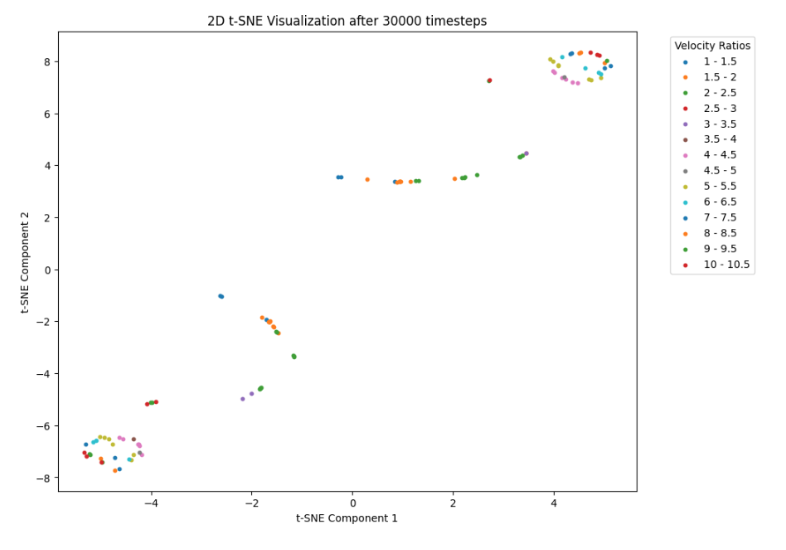
\includegraphics[width=15cm]{images/Clustering/tsne.png}
    \caption{Scatter plot presenting a 2D t-SNE visualization of steady-state simulation data at 30000 time-steps, categorized by varying velocity ratios. Each dot on the plot represents a simulation data point, and the color coding corresponds to different ranges of velocity ratios, from 1-1.5 up to 10-10.5, as detailed in the legend.}
    \label{tsne}
    \end{figure}

The application of DBSCAN to these reduced-dimensional representations led to the identification of distinct flow behavior clusters, categorized based on jet deflection and Coanda adhesion phenomena.\\
While there are not any discernible patterns for the transient data, we observe clear structures and patterns emerging for steady-state data. 
The implementation of unsupervised learning techniques, from dimensionality reduction to clustering, unveils the nuanced patterns hidden within CFD simulation data. The subsequent dimensionality reduction by PCA and t-SNE reduced data undergoes DBSCAN clustering. This presents distinguishable clusters which are indicative of the steady-state data's flow behavior patterns. An examination of the scatter plot (Figure \ref{fig:dbscan_results}) reveals the emergence of three distinct clusters:

\begin{itemize}
  \item \textbf{Blue Cluster (Coanda Adhesion to the Top Surface):} The blue cluster, isolated in the lower quadrant of the plot and denoted by a blue ring, likely represents instances of Coanda adhesion to the top surface of the nozzle. The spatial separation of these points from the central mass suggests a specific, consistently observed flow behavior across these simulations.
  \item \textbf{Yellow Cluster (Coanda Adhesion to the Bottom Surface):} The cluster circled in yellow, situated in the upper right of the plot, corresponds to the simulations exhibiting Coanda adhesion to the bottom surface. The compactness and isolated location of this cluster signify a distinct and strong pattern of flow behavior.
  \item \textbf{Violet Points (Jet Deflection):} The violet points, dispersed between the blue and yellow clusters, likely characterize scenarios where the jet deflects towards either surface, representing a transitional behavior that does not culminate in pronounced Coanda adhesion.
\end{itemize}

\begin{figure}[ht]
\centering
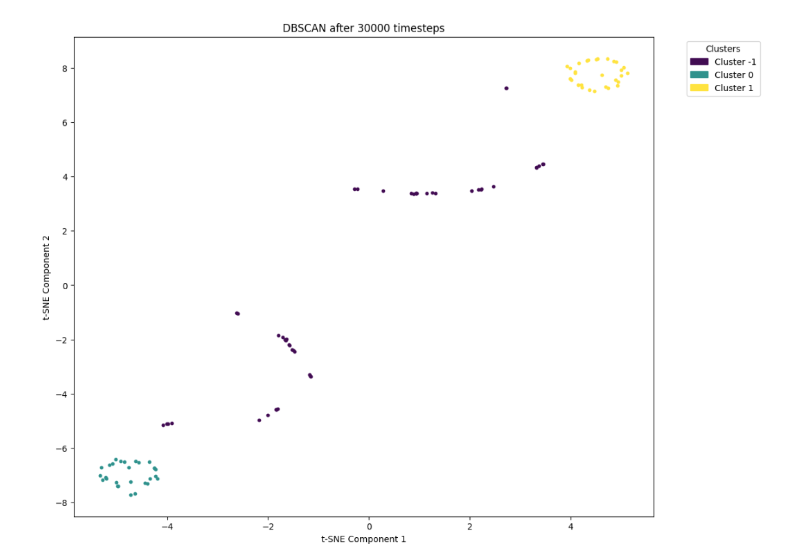
\includegraphics[width=15cm]{images/Clustering/cluster1.png}
\caption{DBSCAN clustering results visualized on t-SNE reduced simulation data after 30000 time-steps.}
\label{fig:dbscan_results}
\end{figure}

This plot substantiates the ability of the steady-state data, in contrast to the transient data, to manifest clear and structured patterns. Each point on the plot corresponds to a sample from the training-validation dataset. The case numbers have been annotated for each of the points and the above hypothesis about clusters is validated by visual inspection of cases, i.e; if the Coanda adhesion has occurred and the direction of jet deflection. The resultant categorization of the flow behaviors, based on the clustering outcomes, underscores the unsupervised learning techniques' utility in gleaning meaningful insights from complex datasets. \\

For the transient data, t-SNE did not reveal any distinct clusters, indicating that at this early stage, the flow behaviors do not exhibit clear patterns or groupings that can be discernibly separated. Similarly, when applying t-SNE and DBSCAN to the latent space representations derived from the GNN encoder as seen in Figure \ref{fig:dbscan_results2}, the resulting clusters were not as prominent or well-defined as those observed within the steady-state data at 30000 time-steps. The latent space clustering outcome suggests that the encoder captures complex high-level features that may not linearly relate to the flow behaviors characterized at steady-state. This observation emphasizes the challenges inherent in extracting clear patterns from dynamic systems in transition and from abstract representations such as the latent space of a GNN.
\begin{figure}[ht]
    \centering
    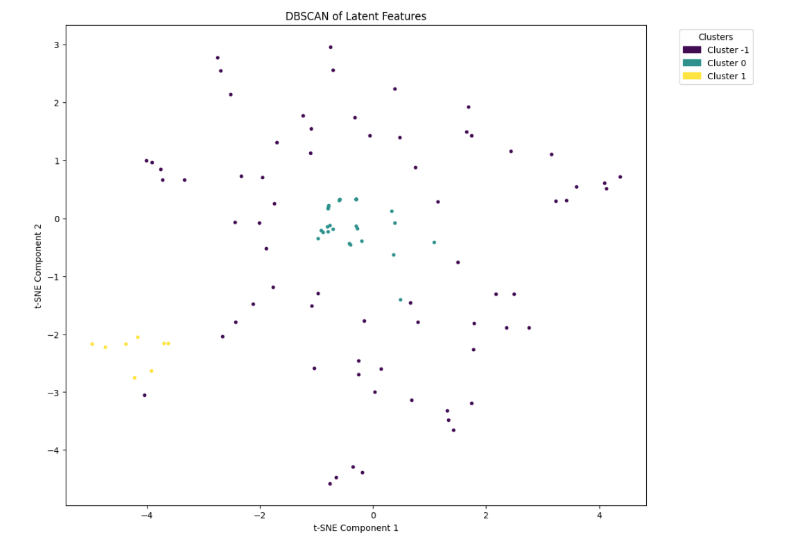
\includegraphics[width=15cm]{images/Clustering/cluster2.png}
    \caption{DBSCAN clustering results visualized on t-SNE reduced latent space vectors.}
    \label{fig:dbscan_results2}
    \end{figure}